\documentclass[12pt, a4paper, oneside]{ctexart}
\usepackage{amsmath, amsthm, amssymb, bm, color, graphicx, geometry, mathrsfs,extarrows, braket, booktabs, array, wrapfig}
\usepackage[colorlinks,linkcolor=red,anchorcolor=blue,citecolor=blue,urlcolor=blue,menucolor=black]{hyperref}
\setCJKmainfont{方正新书宋_GBK.ttf}[ BoldFont = 方正小标宋_GBK, ItalicFont = 方正楷体_GBK]
\setmainfont{Times New Roman}  % 设置英文字体
\setsansfont{Calibri}
\setmonofont{Consolas}

\linespread{1.4}
%\geometry{left=2.54cm,right=2.54cm,top=3.18cm,bottom=3.18cm}
\geometry{left=1.84cm,right=1.84cm,top=2.18cm,bottom=2.18cm}
\newcounter{problem}  % 问题序号计数器
\newenvironment{problem}[1][]{\stepcounter{problem}\par\noindent\textbf{题目\arabic{problem}. #1}}{\smallskip\par}
\newenvironment{solution}[1][]{\par\noindent\textbf{#1解答. }}{\smallskip\par}  % 可带一个参数表示题号\begin{solution}{题号}
\newenvironment{note}{\par\noindent\textbf{注记. }}{\smallskip\par}

%%%% 图片相对路径 %%%%
\graphicspath{{figure/}} % 当前目录下的figure文件夹, {../figure/}则是父目录的figure文件夹

\everymath{\displaystyle} % 默认全部行间公式
\DeclareMathOperator*\uplim{\overline{lim}} % 定义上极限 \uplim_{}
\DeclareMathOperator*\lowlim{\underline{lim}} % 定义下极限 \lowlim_{}
\let\leq=\leqslant % 将全部leq变为leqslant
\let\geq=\geqslant % geq同理

%%%% 一些宏定义 %%%%
\def\bd{\boldsymbol}        % 加粗(向量) boldsymbol
\def\disp{\displaystyle}    % 使用行间公式 displaystyle(默认)
\def\tsty{\textstyle}       % 使用行内公式 textstyle
\def\sign{\text{sign}}      % sign function
\def\wtd{\widetilde}        % 宽波浪线 widetilde
\def\R{\mathbb{R}}          % Real number
\def\N{\mathbb{N}}          % Natural number
\def\Z{\mathbb{Z}}          % Integer number
\def\Q{\mathbb{Q}}          % Rational number
\def\C{\mathbb{C}}          % Complex number
\def\K{\mathbb{K}}          % Number Field
\def\P{\mathbb{P}}          % Polynomial
\def\d{\mathrm{d}}          % differential operator
\def\e{\mathrm{e}}          % Euler's number
\def\i{\mathrm{i}}          % imaginary number
\def\re{\mathrm{Re}}        % Real part
\def\im{\mathrm{Im}}        % Imaginary part
\def\res{\mathrm{Res}}      % Residue
\def\ker{\mathrm{Ker}}      % Kernel
\def\L{\mathcal{L}}         % Loss function
\def\wdh{\widehat}          % 宽帽子 widehat
\def\ol{\overline}          % 上横线 overline
\def\ul{\underline}         % 下横线 underline
\def\add{\vspace{1ex}}      % 增加行间距
\def\del{\vspace{-1.5ex}}   % 减少行间距

%%%% 定理类环境的定义 %%%%
\newtheorem{theorem}{定理}

%%%% 基本信息 %%%%
\newcommand{\RQ}{\today} % 日期
\newcommand{\km}{泛函分析} % 科目
\newcommand{\bj}{强基数学002} % 班级
\newcommand{\xm}{吴天阳} % 姓名
\newcommand{\xh}{2204210460} % 学号

\begin{document}

%\pagestyle{empty}
\pagestyle{plain}
\vspace*{-15ex}
\centerline{\begin{tabular}{*5{c}}
    \parbox[t]{0.25\linewidth}{\begin{center}\textbf{日期}\\ \large \textcolor{blue}{\RQ}\end{center}} 
    & \parbox[t]{0.2\linewidth}{\begin{center}\textbf{科目}\\ \large \textcolor{blue}{\km}\end{center}}
    & \parbox[t]{0.2\linewidth}{\begin{center}\textbf{班级}\\ \large \textcolor{blue}{\bj}\end{center}}
    & \parbox[t]{0.1\linewidth}{\begin{center}\textbf{姓名}\\ \large \textcolor{blue}{\xm}\end{center}}
    & \parbox[t]{0.15\linewidth}{\begin{center}\textbf{学号}\\ \large \textcolor{blue}{\xh}\end{center}} \\ \hline
\end{tabular}}
\begin{center}
    \zihao{-3}\textbf{第六次作业}
\end{center}
\vspace{-0.2cm}
% 正文部分
\begin{problem}[(1.6.2)]
    求证:在$C[a,b]$中不可能引进一种内积$(\cdot ,\cdot)$,使其满足
    \begin{equation*}
        (f,f)^{\frac{1}{2}} = \max_{a\leq x\leq b}|f(x|),\quad(\forall f\in C[a,b]).
    \end{equation*}
\end{problem}\vspace*{-1cm}
\begin{proof}
    令$f(x) = \frac{x-b}{a-b} + \frac{1}{3}\cdot\frac{x-a}{b-a},\ g(x) = \frac{1}{3}\frac{x-a}{b-a}$,则$||f|| = 1,\ ||g|| = \frac{1}{3}$,且
    \begin{equation*}
        f+g = \frac{x-b}{a-b}+\frac{2}{3}\frac{x-a}{b-a},\ f-g = \frac{x-b}{a-b},
    \end{equation*}
    于是$||f+g|| = ||f-g|| = 1$,则$||f+g||^2+||f-g||^2 = 2\neq 2(\frac{1}{3^2}+1) = 2(||f||^2+||g||^2)$,故范数不满足平行四边形公式,无法构成内积.
\end{proof}
\begin{problem}[(1.6.3)]
    在$L^2[0,T]$中,求证:函数
    \begin{equation*}
        x\mapsto \left|\int_0^T\e^{-(T-\tau)}x(\tau)\,\d \tau\right|\quad(\forall x\in L^2[0,T])
    \end{equation*}
    在单位球面上达到最大值,求出此时的最大值和达到最大值的元素$x$.
\end{problem}
\begin{proof}
    \begin{equation*}
        \left|\int_0^T\e^{-(T-\tau)}x(\tau)\,\d \tau\right|\leq \left(\int_0^T\e^{-2(T-\tau)}\,\d \tau\right)^{\frac{1}{2}}\left(\int_0^T|x|^2\,\d \tau\right)^{\frac{1}{2}} = \left(\int_0^T\e^{-2\tau}\,\d \tau\right)^{\frac{1}{2}} = \sqrt{\frac{1-\e^{-2T}}{2}}
    \end{equation*}
    上式取到最大值,当且仅当$\exists \lambda\in \R$,使得$x = \lambda \e^{-(T-\tau)}$且$\int_0^T|x|^2\,\d\tau = 1$,于是
    \begin{equation*}
        \int_0^T|x|^2\,\d \tau = \lambda^2\int_0^T\e^{-2(T-\tau)}\,\d \tau = \lambda^2\int_0^T\e^{-2\tau}\,\d \tau = \lambda^2\frac{1-\e^{-2T}}{2} = 1
    \end{equation*}
    所以$\lambda = \pm\sqrt{\frac{2}{1-\e^{-2T}}}$,故$x$能在单位球面上取到最大值,且当$x = \pm\sqrt{\frac{2}{1-\e^{-2T}}}\e^{-(T-\tau)} = \pm\sqrt{\frac{2}{\e^{2T}-1}}\e^\tau$时取到最大值$\sqrt{\frac{1-\e^{-2T}}{2}}$.
\end{proof}
\begin{problem}[(1.6.5)]
    设$M$是Hilbert空间$X$的子集,求证:$(M^{\perp})^{\perp} = \overline{\text{span}M}$.
\end{problem}
\begin{proof}
    由于$\overline{\text{span}M} = ((\text{span}M)^{\perp})^{\perp}$,于是只需证$((\text{span}M)^{\perp})^{\perp} = (M^\perp)^\perp$,只需证$(\text{span}M)^{\perp} = M^{\perp}$,由于$M\subset \text{span}M$,则$(\text{span}M)^\perp\subset M^\perp$.

    $\forall x\in M^\perp$,$\forall y\in\text{span}M$,则$\exists u\in \N, \alpha_i\in \K, x_i\in M$,使得$y = \sum_{i=1}^n\alpha_ix_i$,则
    \begin{equation*}
        (y,x) =(\sum_{i=1}^n\alpha_ix_i, x) = \sum_{i=1}^n\alpha_i(x_i,x) = 0
    \end{equation*}
    则$x\in (\text{span}M)^\perp$,则$(\text{span}M)^\perp = M^\perp$.
\end{proof}
\begin{problem}[(1.6.6)]
    在$L^2[-1,1]$中,问偶函数集的正交补是什么?
\end{problem}
\begin{solution}
    偶函数的正交补为奇函数. 令全体偶函数集合为$M$,由于$\{\sin n\pi x,\cos n\pi x\}_{n\geq 0}$是$L^2[-1,1]$上的完备标准正交基. $\forall f \in M^T$,则$(f,\cos n\pi x) = 0,\ (n\geq 0)$,于是$f= \sum_{i=1}^\infty (f, \sin n\pi x)\sin n\pi x$,所以$f$是奇函数,由$f$的任意性可知,$M^T$是奇函数集合.
\end{solution}
\begin{problem}[(1.6.7)]
    在$L^2[a,b]$中,考察函数集$S = \{\e^{2\pi \i nx}\}$.

    (1) 若$|b-a|\leq 1$,求证:$S^\perp = \{\theta\}$.

    (2) 若$|b-a| > 1$,求证:$S^\perp\neq \{\theta\}$.
\end{problem}
\begin{proof}
    (1) 当$b-a=1$时,$S^\perp = (\text{span}S)^\perp = L^2[a,b]^\perp = \{\theta\}$.

    当$b-a < 1$时,$\forall u\in L^2[a,b]$,令$\bar{u} = \begin{cases}
        u,&\quad x\in [a,b],\\ 0,&\quad x\in (b,a+1]
    \end{cases}$即为$u$在$[a,b]$上的零延拓. 则$\bar{u}\in L^2[a,a+1]$. 若$(u, \e^{2\pi \i nx}) = 0$,则
    \begin{equation*}
        \int_a^bu\e^{2\pi\i nx}\,\d x = \int_a^{a+1}\bar{u}\e^{2\pi inx}\,\d x = 0,\quad(\forall n\in \Z)
    \end{equation*}

    (2) 当$b-a > 1$时,令$u_n = -\int_{a+1}^b\e^{2\pi\i nx}\,\d x$,下证$\{u_n\}\in l^2$. 
    \begin{equation*}
        |u_n| = \left|\int_{a+1}^b\e^{2\pi\i nx}\,\d x\right|=\left|\frac{1}{2\pi\i n}\left(\e^{2\pi\i nb}-\e^{2\pi\i n(a+1)}\right)\right| = \frac{1}{2\pi n}\left|\e^{2\pi\i nb}-\e^{2\pi\i n(a+1)}\right|\leq \frac{1}{\pi n}.
    \end{equation*}
    于是$\sum_{n=1}^\infty |u_n|^2\leq \sum_{n=1}^\infty \frac{1}{(\pi n)^2} < \infty$,则$\sum_{n=-\infty}^\infty |u_n|^2\leq 2\sum_{n=1}^\infty |u_n|^2 + (b-a-1)^2 < \infty$,所以$\{u_n\}\in l^2$.
    
    由于$S$在$L^2[a,a+1]$上完备,由Riesz-Fisher定理知$u = \sum_{n=-\infty}^\infty u_n\e^{2\pi \i nx}\in L^2[a,a+1]$,则令$v = \begin{cases}
        u,&\quad x\in [a,a+1],\\
        1,&\quad x\in (a+1,b].
    \end{cases}$于是$\forall n\in \Z$有
    \begin{equation*}
        (v, \e^{2\pi \i nx}) = \int_a^bv\e^{2\pi\i nx}\,\d x = \int_a^{a+1}u\e^{2\pi \i nx}\,\d x + \int_{a+1}^b\e^{2\pi \i nx}\,\d x = u_n + \int_{a+1}^b \e^{2\pi\i n x}\,\d x= 0
    \end{equation*}
    则$v\in S^{\perp}$且$v\neq \theta$,则$S^\perp\neq {\theta}$.
\end{proof}
\begin{problem}[(1.6.8)]
    设$X$表示闭单位园上的解析函数全体,内积定义为
    \begin{equation*}
        (f,g) = \frac{1}{\i}\oint_{|z| = 1}\frac{f(x)\ol{g(z)}}{z}\,\d z\quad(\forall f,g\in X)
    \end{equation*}
    求证:$\{z^n/\sqrt{2\pi}\}$是一组标准正交系.
\end{problem}
\begin{proof}不妨令$n > m$.
    \begin{align*}
        (\frac{z^n}{\sqrt{2\pi}}, \frac{z^n}{\sqrt{2\pi}}) =&\ \frac{1}{2\pi \i}\int_{|z|=1}\frac{(z\bar{z})^n}{z}\,\d z = \frac{1}{2\pi \i}\int_{|z| = 1}\frac{|z|^{2n}}{z}\,\d z = \frac{1}{2\pi\i}\int_{|z| = 1}\frac{1}{z}\,\d z = 1,\\
        (\frac{z^n}{\sqrt{2\pi}}, \frac{z^m}{\sqrt{2\pi}}) =&\ \frac{1}{2\pi\i}\int_{|z| = 1}\frac{z^n\bar{z}^m}{z}\,\d z = \frac{1}{2\pi \i}\int_{|z|=1}z^{n-1}\bar{z}^m\,\d z = 0.
    \end{align*}
    故$\{z^n/\sqrt{2\pi}\}$是一组标准正交系.
\end{proof}
\begin{problem}[(1.6.9)]
    设$\{e_n\}_{n=1}^\infty, \{f_n\}_{n=1}^\infty$是Hilbert空间$X$中的两个规范正交系,满足条件
    \begin{equation*}
        \sum_{n=1}^\infty ||e_n-f_n||^2 < 1.
    \end{equation*}
    求证:$\{e_n\}$和$\{f_n\}$两者中一个完备蕴含另一个完备.
\end{problem}
\begin{proof}
    设$\{e_n\}$完备的,由于$X$为Hilbert空间,则完备性与完全性等价. 反设,$\exists x_0\in X$,且$x_0\neq 0$,使得$(x_0,f_n) = 0,\ (n\geq 1)$则
    \begin{align*}
        &\ |(x_0,e_n)| = |(x_0,e_n-f_n)| \leq ||x_0||\cdot ||e_n-f_n||\\
        \Rightarrow&\ \sum_{n=1}^\infty |(x_0,e_n)| = ||x_0||^2\leq ||x_0||^2\sum_{n=1}^\infty||e_n-f_n|| < ||x_0||^2
    \end{align*}
    矛盾,故$\{f_n\}$完备.
\end{proof}
\begin{problem}[(1.6.10)]
    设$X$是Hilbert空间,$X_0$是$X$的闭线性子空间,$\{e_n\},\{f_n\}$分别是$X_0$和$X_0^\perp$的规范正交系. 求证:$\{e_n\}\cup\{f_n\}$是$X$的规范正交系.
\end{problem}
\begin{proof}
    由于$\{e_n\},\{f_n\}$为标准正交系,$\forall n,m\geq 1,\ n\neq m$,则$|(e_n,e_n)| = |(f_n,f_n)| = 1$,$e_n\perp e_m,\ f_n\perp f_m$,由于$e_n\in X_0$,$f_m\in X_0^\perp$,则$e_n\perp f_m$. 综上$\{e_n\}\cup \{f_n\}$是$X$的标准正交系.
\end{proof}
\begin{problem}[(1.6.12)]
    设$X$是内积空间,$\{e_n\}$是$X$中的规范正交系,求证:
    \begin{equation*}
        \left|\sum_{n=1}^\infty (x,e_n)\ol{(y,e_n)}\right|\leq ||x||\cdot||y||\quad(\forall x, y\in X).
    \end{equation*}
\end{problem}\vspace*{-1cm}
\begin{proof}
    \begin{equation*}
        \left|\sum_{n=1}^\infty(x,e_n)\ol{(y,e_n)}\right|^2\leq \left(\sum_{n=1}^\infty|(x,e_n)|^2\right)\left(\sum_{n=1}^\infty|(y,e_n)|^2\right)\leq ||x||^2\cdot||y||^2
    \end{equation*}
    于是$\left|\sum_{n=1}^\infty (x,e_n)\ol{(y,e_n)}\right|\leq ||x||\cdot||y||\quad(\forall x, y\in X)$.
\end{proof}
\begin{problem}[(1.6.13)]
    设$X$是一个内积空间,$\forall x_0\in X,\forall r > 0$,令
    \begin{equation*}
        C = \{x\in X:||x-x_0|| \leq r\}.
    \end{equation*}

    (1) 求证:$C$是$X$中的闭凸集.

    (2) $\forall x\in X$,令
    \begin{equation*}
        y = \begin{cases}
            x_0+r\frac{x-x_0}{||x-x_0||},&\quad x\notin C,\\
            x,&\quad x\in C.
        \end{cases}
    \end{equation*}
    求证:$y$是$x$在$C$中的最佳逼近元.
\end{problem}
\begin{proof}
    (1) 设$\{x_n\}\in C$收敛于$x$,则
    \begin{equation*}
        ||x-x_0||\leq ||x-x_n|| + ||x_n-x_0||\leq ||x-x_n||+r\to r\quad(n\to\infty)
    \end{equation*}
    则$x\in C$,由$\{x_n\}$的任意性知$C$是闭的.

    $\forall \alpha \in (0,1)$,$x,y\in C$,则$||x-x_0||\leq r,\ ||y-x_0||\leq r$,则
    \begin{equation*}
        ||\alpha x+(1-\alpha)y-x_0|| = ||\alpha(x-x_0)+(1-\alpha)(y-x_0)||\leq \alpha||x-x_0||+(1-\alpha)||y-x_0||\leq r
    \end{equation*}
    则$\alpha x+(1-\alpha)y\in C$,故$C$是$X$的闭凸子集.

    (2) 当$x\in C$时,$||y-x|| = 0$,则$y$是$x$的最佳逼近元.

    当$x\notin C$时,
    \begin{equation*}
        ||x-y|| = \left|\left|x-x_0-r\frac{x-x_0}{||x-x_0||}\right|\right| = \left|\left|\frac{||x-x_0||-r}{||x-x_0||}(x-x_0)\right|\right| = ||x-x_0||-r
    \end{equation*}
    由于$\forall z\in C$有$||z-x||+r\geq ||z-x||+||z-x_0|| \geq ||x-x_0||$,则$||z-x||\geq ||x-x_0||-r = ||x-y||$,又由于$C$是闭的,则
    \begin{equation*}
        ||x-y||=\inf_{z\in C}||z-x|| = \rho(x, C)
    \end{equation*}
    则$y$是$x$在$C$中的最佳逼近元.
\end{proof}
\begin{problem}[(1.6.14)]
    求$(a_0,a_1,a_2)\in \R^3$,使得$\int_0^1|\e^t-a_0-a_1t-a_2t^2|^2\,\d t$取最小值.
\end{problem}
\begin{solution}
    等价于$\e^t$在空间$\text{span}\{1,t,t^2\}$上的正交投影,即
    \begin{equation*}
        \begin{cases}
            a_0(1,1)+a_1(t,1)+a_2(t^2,1)=(\e^t,1),\\
            a_0(1,t)+a_1(t,t)+a_2(t^2,t)=(\e^t,t),\\
            a_0(1,t^2)+a_1(t,t^2)+a_2(t^2,t^2)=(e^t,t^2).
        \end{cases}\Rightarrow\left[\begin{matrix}
            1&1/2&1/3\\
            1/2&1/3&1/4\\
            1/3&1/4&1/5
        \end{matrix}\right]\left[\begin{matrix}
            a_0\\a_1\\a_2
        \end{matrix}\right] = \left[\begin{matrix}
            \e-1\\1\\e-2
        \end{matrix}\right]
    \end{equation*}
    则$a_0 = 39\e-105,\ a_1 = 588-216\e,\ a_2 = 210\e-570$.
\end{solution}
\begin{problem}[(1.6.15)]
    设$f(x)\in C^2[a,b]$,满足边界条件
    \begin{equation*}
        f(a)=f(b) = 0,\quad f'(a)=  1,\ f'(b) = 0.
    \end{equation*}
    求证:
    \begin{equation*}
        \int_a^b|f''(x)|^2\,\d x \geq \frac{4}{b-a}.
    \end{equation*}
\end{problem}
\begin{problem}
    令$(\alpha_1T_1+\alpha_2T_2)(x) = \alpha_1T_1(x)+\alpha_2T_2(x)$,则$L(X, Y)$构成线性空间,证明在算子范数下构成$B^*$空间.
\end{problem}
\begin{proof}
    正定性:$||T|| = \sup_{\substack{x\in D(T)\\ x\neq \theta}}\frac{||Tx||}{||x||}\geq 0$,且$||T|| = 0\iff ||Tx|| = 0\iff Tx = \theta\iff T = \theta$.\add

    齐次性:$\forall \alpha \in \K$,则$||\alpha T|| = \sup_{\substack{x\in D(T)\\ x\neq \theta}}\frac{||(\alpha T)(x)||}{||x||} = \sup_{\substack{x\in D(T)\\ x\neq \theta}}\frac{||\alpha T(x)||}{||x||} = |\alpha|\cdot ||T||$.\add

    三角不等式:
    \begin{equation*}
        ||T_1+T_2|| = \sup_{\substack{x\in D(T)\\ x\neq \theta}}\frac{||(T_1+T_2)(x)||}{||x||} = \sup_{\substack{x\in D(T)\\ x\neq \theta}}\frac{||T_1(x)+T_2(x)||}{||x||}\leq \sup_{\substack{x\in D(T)\\ x\neq \theta}}\frac{||T_1||}{||x||}+\sup_{\substack{x\in D(T)\\ x\neq \theta}}\frac{||T_2||}{||x||} = ||T_1||+||T_2||
    \end{equation*}

    综上,$L(X,Y)$在算子范数系构成$B^*$空间.
\end{proof}
\begin{problem}
    设$X$是$B^*$空间,$f$是$X$中的线性泛函. 证明$f$连续$\iff\ker f$是$X$中的闭子空间.
\end{problem}
\begin{proof}
    必要性:设$\{x_n\}\subset \ker f$收敛于$x$,则$f(x_n) = 0$,所以$\lim_{n\to\infty}f(x_n) = 0$,所以$\lim_{n\to\infty}f(x_n) = f(x) = 0$,则$x\in \ker f$,故$\ker f$是闭的.

    $\forall \alpha,\beta\in \K,\forall x, y\in \ker f$,则$f(\alpha x+\beta y) = \alpha f(x) + \beta f(y) = 0$,故$\alpha x+\beta y\in \ker f$. 综上,$\ker f$是$X$的闭子空间.

    充分性:由于$f$连续等价于$f$在单位球面上有界,反设$f$在单位球面上无界,则$\forall n\in \N$,$\exists x_n\in X$且$||x_n|| = 1$,$f(x_n) \geq n\Rightarrow \frac{1}{n}\geq \frac{1}{f(x_n)}$,令$y_n = \frac{x_n}{f(x_n)} - \frac{x_1}{f(x_1)}$,则
    \begin{equation*}
        \left|\left|y_n+\frac{x_1}{f(x_1)}\right|\right| = \left|\left|\frac{x_n}{f_n}\right|\right| = \frac{1}{f(x_n)}\leq \frac{1}{n}\to 0\quad(n\to\infty)
    \end{equation*}
    则$y_n\to-\frac{x_n}{f(x_1)}$,且$f(y_n) = 0$,则$\{y_n\}\subset \ker f$收敛,但是$f(-\frac{x_1}{f(x_1)}) = -1\neq 0$,则$-\frac{x_1}{f(x_1)}\notin \ker f$与$\ker f$是闭的矛盾. 故$f$在单位球面上有界,$f$连续.
\end{proof}

% 下面给一些功能的写法
\iffalse
% 图片模板
\centerline{
    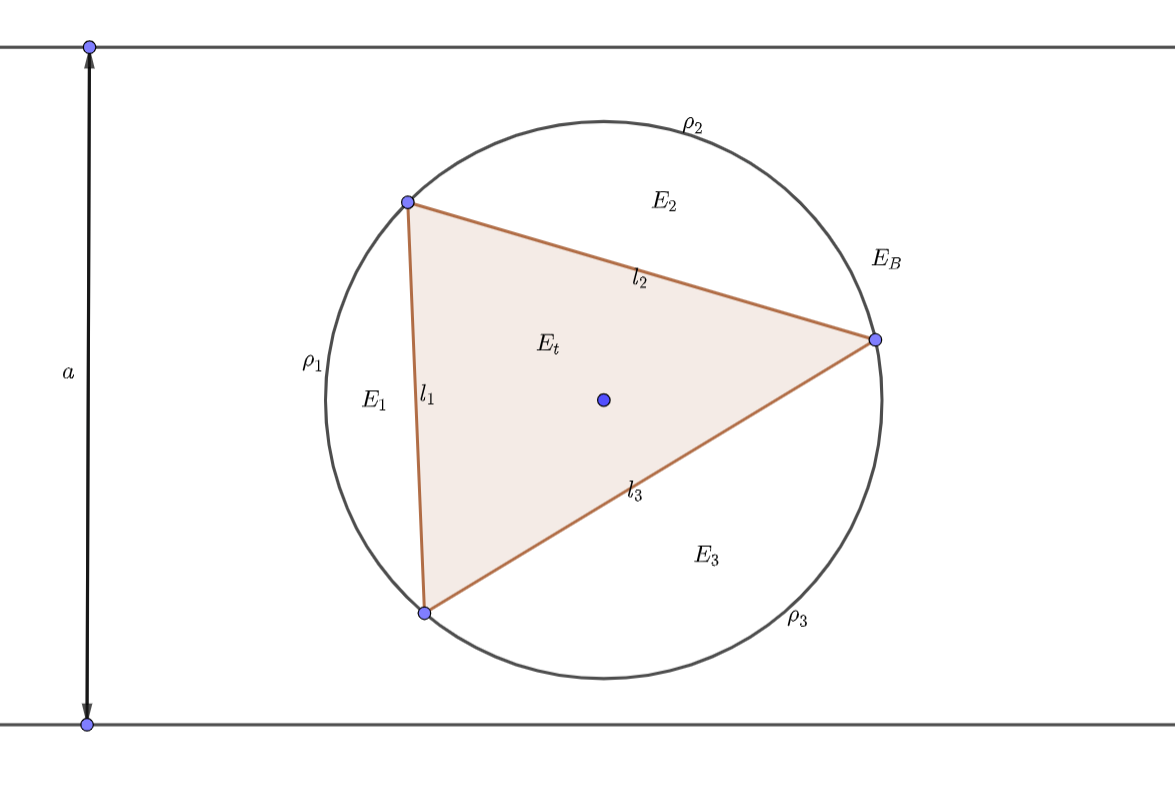
\includegraphics[width=0.8\textwidth]{figure.png}
}
% 表格模板
\renewcommand\arraystretch{0.8} % 设置表格高度为原来的0.8倍
\begin{table}[!htbp] % table标准
    \centering % 表格居中
    \begin{tabular}{p{1cm}<{\centering}p{1cm}<{\centering}p{3cm}<{\centering}p{5cm}<{\centering}} % 设置表格宽度
    %\begin{tabular}{cccc}
        \toprule
        $x_i$ & $f[x_1]$ & $f[x_i,x_{i+1}]$ & $f[x_i,x_{i+1},x_{i+2}]$ \\
        \midrule
        $x_0$ & $f(x_0)$ &                  &                          \\
        $x_0$ & $f(x_0)$ & $f'(x_0)$        &                          \\
        $x_0$ & $f(x_1)$ & $\frac{f(x_1)-f(x_0)}{x_1-x_0}$ & $\frac{f(x_1)-f(x_0)}{(x_1-x_0)^2}-\frac{f'(x_0)}{x_1-x_0}$\\
        \bottomrule
    \end{tabular}
\end{table}

\def\Log{\text{Log}} % 一个简单的宏定义
$\Log$ % 调用方法
\fi

\end{document}